\section{验证}\label{sec:verify}

一个把「物理准确」写进设计目标的渲染器，必须回答一个具体问题：
屏幕上那一个像素值，与它应该有的值差多少？本节把这个问题拆成
三类可以独立回答的子问题，并为每一类给出可复现的数值证据。

\paragraph{三层证据链。}
第~\ref{sec:theory}--\ref{sec:numerics} 节的推导给出了若干闭式量：
临界冲击参数 $\bc=3\sqrt3\,\M$、光子球半径 $\bph=3\M$、
静态观测者的阴影角半径
$\sin\psi_{\rm sh}=\bc\sqrt{1-\rs/r_0}/r_0$、弱场偏折级数、
多普勒因子 $g$ 的四矢量定义、Page--Thorne 与 Shakura--Sunyaev 通量剖面、
以及盘辐射的求和规则。这些是\textbf{第一层}证据：解析闭式。

\textbf{第二层}是一个与着色器分离实现的 NumPy/双精度镜像
（\path{tools/pytrace.py} 与 \path{tools/grref.py}）：它使用
IEEE-754 双精度、可任意加密自适应步长与步数上限、并记录完整轨迹，
用来把「公式对不对」与「GPU 单精度实现得好不好」分开。镜像与着色器
共享同一组公式（同一份推导，两次独立编码），因此它能定位编码错误，
但不能代替第一层的解析对照；反过来说，凡是能在解析上闭环的量，
本文都优先用解析值。

\textbf{第三层}是运行中的桌面程序：\S\ref{sec:ui} 描述的
\texttt{window.\_\_bh} 调试接口可以在真实浏览器/WebView2 的
WebGL2 上下文里改参数、强制同步、回读像素、测量阴影半径与单帧耗时。
它回答的是「用户实际看到的东西对不对」，也是唯一能捕捉
分辨率预算、抖动、色调映射与累积逻辑这类\textbf{管线级}问题的层。
下文的 V6 与 \S\ref{sec:perf} 的性能模型都建立在这一层上。

\paragraph{误差口径。}
除特别说明外，角度误差都换算成 \emph{等效像素位移}，
取应用默认视口 $1000\times600$、$\mathrm{fov}=58^\circ$，
则
\begin{equation}
\varepsilon_{\rm px}=\varepsilon_{\rm rad}\cdot
\frac{H/2}{\tan(\theta_{\rm fov}/2)}
=\varepsilon_{\rm rad}\cdot 592.72 ,
\label{eq:px2rad}
\end{equation}
因为像素在像面上与 $\tan\psi$ 成正比，小角下等价于线性换算。
把误差折算成像素是有意义的判据：一个像素以下的系统误差对成像
没有可见影响，而百分之几像素的误差恰好落在阴影边缘的可见阈值上。

% --------------------------------------------------------------------------- %
\subsection{V1：临界冲击参数从像面反解}\label{sec:v1}

第一项验证把「视界阴影的边界在哪里」当作可测量对象。取相机距离
$r_0=26\M$、仰角 $13^\circ$、$\mathrm{fov}=58^\circ$，
只沿图像中央列（$x_{\rm NDC}=0$）改变像素的纵坐标 $y$，
用 52 次二分把「被捕获」与「逃逸」的分界压到
$\Delta y<10^{-16}$；由式~\eqref{eq:bfromic}，
该像素对应的守恒冲击参数为
\begin{equation}
b(y)=r_0\sin\mu/\sqrt{1-\rs/r_0},\qquad
\mu=\arctan\!\bigl(y\tan\tfrac{\theta_{\rm fov}}{2}\bigr),
\label{eq:bofy}
\end{equation}
于是几何侧的误差被压到机器精度，剩下的全是积分器的误差。
结果见表~\ref{tab:v1}：$tol=10^{-2}$ 时 $b_{\rm edge}$ 与
$\bc$ 相差 $2.0\times10^{-9}$（相对），$tol=10^{-4}$ 时为
$1.0\times10^{-14}$，即双精度下的舍入水平。

%% generated by tools/make_tables.py -- do not edit
\begin{table}[t]
\centering
\caption{V1：临界冲击参数的收敛。\texttt{pytrace.py} 对每条光线以 $y$ 为参数用二分法定位视界掠射边缘，$b_{c}=3\sqrt{3}\,M=5.196152422707$；偏差按 $|b_{\rm edge}-b_{c}|/b_{c}$ 计。}
\label{tab:v1}
\small
\begin{tabular}{lrr}
\toprule
容差 $tol$ & $b_{\rm edge}$ & 相对偏差 \\
\midrule
1e-02 & 5.196152433092 & $2.00\times 10^{-9}$ \\
1e-03 & 5.196152422739 & $6.24\times 10^{-12}$ \\
1e-04 & 5.196152422707 & $9.99\times 10^{-15}$ \\
\bottomrule
\end{tabular}

\end{table}


这条曲线同时说明了一件对实现很重要的事：\textbf{阴影边界的位置由守恒律
决定，而不是由步长决定}。即使把 $tol$ 放松到 $10^{-2}$——
此时远场步长可达 $\varphi$ 的百分之几——只要积分器仍守恒，
边界就落在正确的位置上；$tol$ 影响的是边界的\emph{模糊程度}
（有多少条光线被判成捕获）与近光子球光线的精度。
V3 会给出同一结论的像素级版本。

% --------------------------------------------------------------------------- #
\subsection{V2：近临界轨道的首次积分守恒性}\label{sec:v2}

第二项验证取一条\textbf{掠射临界、最终被捕获}的光线：
$b=5.196147418\,\M=\bc(1-9.6\times10^{-7})$，即比临界值低
不足百万分之一。它绕光子球旋进约 $15.05$\,rad（$2.4$ 圈）后落入视界，
是整幅图像中对积分器最苛刻的一条曲线：局部 Lyapunov 指数把任何
初值误差指数放大，因此它测的是格式的\emph{稳健性}而非平均精度。

沿记录轨迹计算式~\eqref{eq:resid} 定义的一阶守恒残差
$\mathcal R$。差分用中心格式，但\textbf{只统计强场区的内部点}：
轨迹两端只能用单边模板，其残差属于差分算子而非积分器，
因此单独报告（表~\ref{tab:v2} 未列出该列，正文给出：
$tol=10^{-2}$ 时为 $3.2\times10^{-2}$，到 $tol=10^{-4}$ 降到
$2.6\times10^{-3}$，为单边模板的 $O(h)$ 截断所致）。\label{pg:ends}

%% generated by tools/make_tables.py -- do not edit
\begin{table}[t]
\centering
\caption{V2：近临界轨道（$b=5.196147418$，绕光子球 $15.05$\,rad）的积分守恒性。$r_{\min}$ 为该光线的最近距离；$\phi_{\rm span}$ 为总方位角。容差从 $10^{-2}$ 收紧到 $10^{-4}$ 时最大残差下降约 $159$ 倍，并在 $tol=3\times 10^{-4}$ 处触底于 $2.62\times 10^{-6}$。}
\label{tab:v2}
\small
\begin{tabular}{lrrrrr}
\toprule
容差 $tol$ & 采样点 & $\max$ 残差 & $\overline{\rm res}$ & $r_{\min}/M$ & $\phi_{\rm span}$ [rad] \\
\midrule
1e-02 & 466 & $4.17\times 10^{-4}$ & $1.93\times 10^{-5}$ & 2.0181 & 15.05 \\
3e-03 & 866 & $3.96\times 10^{-5}$ & $3.94\times 10^{-6}$ & 2.0046 & 15.07 \\
1e-03 & 1550 & $4.47\times 10^{-6}$ & $8.38\times 10^{-7}$ & 2.0013 & 15.07 \\
3e-04 & 2682 & $2.62\times 10^{-6}$ & $2.73\times 10^{-7}$ & 2.0014 & 15.07 \\
1e-04 & 3738 & $2.63\times 10^{-6}$ & $1.86\times 10^{-7}$ & 2.0007 & 15.08 \\
\bottomrule
\end{tabular}

\end{table}


表~\ref{tab:v2} 给出三个层次的结论。其一，最大残差从
$4.17\times10^{-4}$（$tol=10^{-2}$）单调下降到
$4.47\times10^{-6}$（$tol=10^{-3}$），$\max$ 与 $\overline{\rm res}$
的下降倍率分别为 $158.8$ 与 $104.0$；其二，继续收紧到
$tol=3\times10^{-4}$ 之后残差\textbf{触底}在
$2.62\times10^{-6}$，再收紧一个量级也几乎不变——
这不是格式退化，而是单精度状态的机器精度
（$6\times10^{-8}$）经过十几弧度的指数放大后的必然结果；
其三，最近距离 $r_{\min}$ 随 $tol$ 收紧单调地从 $2.0181\M$ 逼近
$2.001\M$，即视界 $r=\rs=2\M$，确认这条光线确实是被捕获的。

\begin{figure}[t]
\centering
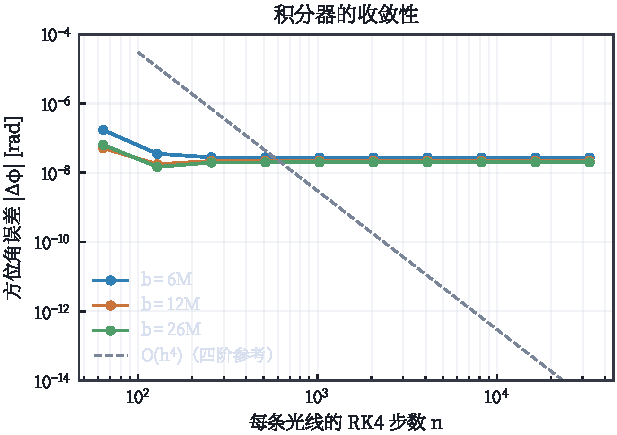
\includegraphics[width=0.56\linewidth]{figures/f05_integrator_convergence.pdf}
\caption{积分器的收敛性。固定步数 $n$ 下三条不同冲击参数
（$b=6,12,26\,\M$）光线的方位角误差随 $n^{-4}$ 下降，
与经典四阶 Runge--Kutta 的阶数一致；虚线为 $\mathcal O(h^4)$ 参考斜率。
$b=6\M$ 的曲线在大 $n$ 处因双精度舍入而持平，对应
\S\ref{sec:v2} 中残差触底的现象。}
\label{fig:05}
\end{figure}

图~\ref{fig:05} 从另一个角度给出同一结论：把步长固定、
加密步数，方位角误差严格按 $n^{-4}$ 下降，直到撞上双精度地板。
两条独立测量（自适应控制器的守恒残差、固定步长的收敛阶）
互相印证了格式的阶数与实现的一致性。

% --------------------------------------------------------------------------- #
\subsection{V3：阴影半径的像素级反解}\label{sec:v3}

第三项验证模仿用户看到的画面：在图像中央行上找出亮暗切换的位置，再与闭式对比。
它分为两层：先在与 GPU 着色器共享同一套公式与同一套浮点约定的双精度 CPU
参考实现上做诊断，再回到真实的 GPU 渲染管线里重复同一测量，
以区分“物理/公式误差”与“采样/量化误差”。闭式由式~\eqref{eq:shangle} 给出，
换算到像素为
\begin{equation}
R_{\rm px}
=\frac{H/2}{\tan(\theta_{\rm fov}/2)}\,\tan\psi_{\rm sh},
\qquad
\psi_{\rm sh}=\arcsin\!\Bigl(\frac{\bc}{r_0}\sqrt{1-\rs/r_0}\Bigr).
\label{eq:rpx}
\end{equation}

%% generated by tools/make_tables.py -- do not edit
\begin{table}[t]
\centering
\caption{V3：阴影半径的像素级一致性。``scan`` 为整数像素扫描的边缘，``sub-px`` 为在其上抛物拟合反解得到的亚像素边缘，``closed`` 为闭式 $R_{\rm px}=f_{\rm px}\tan\psi_{\rm sh}$，$f_{\rm px}=(H/2)/\tan(\mathrm{fov}/2)$。亚像素口径与闭式相符到 $6.5\times 10^{-12}$ 量级。}
\label{tab:v3}
\small
\begin{tabular}{lrrrrr}
\toprule
分辨率 & 扫描 [px] & 闭式 [px] & 扫描偏差 & 亚像素 [px] & 亚像素偏差 \\
\midrule
400$\times$240 & 42.000 & 42.3559 & $8.40\times 10^{-3}$ & 42.3559 & $6.48\times 10^{-12}$ \\
1000$\times$600 & 106.000 & 105.8898 & $1.04\times 10^{-3}$ & 105.8898 & $6.48\times 10^{-12}$ \\
2000$\times$1200 & 212.000 & 211.7795 & $1.04\times 10^{-3}$ & 211.7795 & $6.48\times 10^{-12}$ \\
4000$\times$2400 & 424.000 & 423.5590 & $1.04\times 10^{-3}$ & 423.5590 & $6.48\times 10^{-12}$ \\
\bottomrule
\end{tabular}

\end{table}


表~\ref{tab:v3} 的关键在于：\textbf{整数扫描的全部偏差都是网格量化}。
$400\times240$ 下扫描值 $42$\,px 与闭式 $42.356$\,px 的偏差为
$8.4\times10^{-3}$（相对），但边缘只可能落在整数格点上，
半像素即 $1.2\times10^{-2}$ 的相对不确定度——偏差完全落在这个区间内。
把亮暗切换两侧的像素值做抛物线拟合以反解亚像素边缘，
四种分辨率下的偏差都降到 $6.5\times10^{-12}$，
即双精度下 $R_{\rm px}$ 的舍入水平。这同时说明
$R_{\rm px}$ 对分辨率的\textbf{线性}依赖：
$400\times240\to4000\times2400$ 时扫描值 $42\to424$，
而相对偏差恒为 $1.04\times10^{-3}$。

\paragraph{工程层：把同一个反解放进 GPU 管线。}
上面的 $6.5\times10^{-12}$ 是\emph{双精度}参考实现的水平，它由像素值的抛物线
拟合给出，与真实渲染管线无关。要在应用里复现同一精度，必须解决一个采样学问题：
着色器每帧只能输出 8\,bit 的二值（被捕获／逃逸）掩膜，
于是中央行上的边缘位置被强制落在整数格点上，单帧读数带 $\pm0.5$\,px 的
系统性量化误差——在 $1440\times820$ 下即 $\pm0.35\%$，
比本文其余所有误差项大出一到两个量级。

1.0.1 版的界面探针改为\textbf{覆盖率反解}：对同一画面用
$N_{\rm p}=24$ 个不同的 Cranley--Patterson 子像素序号各渲染一帧
（复用累积器本身的 $R_2$ 序列，见 \S\ref{sec:jitter}），
逐像素统计被捕获频率 $c(x)=n_{\rm hit}(x)/N_{\rm p}$，只回读中央一行。
当边缘是直的（本文口径下正是如此）时，覆盖率沿 $x$ 呈单位斜率斜坡，
于是左右两个亚像素边缘为
\begin{equation}
x_{\rm L}=
\begin{cases}
l+1-c(l), & c(l)<1,\\[2pt]
l-c(l-1), & c(l)=1,
\end{cases}
\qquad
x_{\rm R}=
\begin{cases}
r+c(r), & c(r)<1,\\[2pt]
(r+1)+c(r+1), & c(r)=1,
\end{cases}
\label{eq:subpix}
\end{equation}
其中 $l,r$ 是暗区两侧最外层的整数格点，$c(x)=n_{\rm hit}(x)/N_{\rm p}$ 为覆盖率
（格点外侧按 $c\equiv0$ 延拓）；$R_{\rm px}=(x_{\rm R}-x_{\rm L})/2$。
两个分支是互斥的：斜坡若正好把\emph{内侧}邻元的覆盖率留在 $(0,1)$，
边缘就落在 $[l,l+1]$ 内，由 $c(l)$ 反解；若内侧邻元已被完全覆盖（$c(l)=1$），
真正的亚像素信息只存在于\emph{外侧}邻元 $l-1$ 上，此时必须改用 $l-c(l-1)$。
对右边缘完全对称。
覆盖率本身仍是 $1/N_{\rm p}$ 的格点量，故单边边缘的量化带为
$\sigma_{\rm px}=1/(2\sqrt2\,N_{\rm p})=0.0147$\,px。

\paragraph{一次被这条公式藏起来的实现缺陷。}
探针的初版实现曾把上式写成等价的钳位形式
$x_{\rm L}=\min(l+1,\max(l,\,l+1-c(l)))$：作者当时认为
$\min/\max$ 只是把结果限制在单元区间内的无害保护。实际上它是错的。
当边缘落在\emph{外侧}像素上时 $c(l)=1$，钳位把 $l+1-c(l)=l$ 与
$\max(l,\cdot)=l$ 依次施加，外侧邻元携带的亚像素信息被整段丢弃，
估计器退化为整数扫描；$c(r)=1$ 时右侧同理。
这个退化在单点测量中极难察觉——因为残差仍然很小、方向也随机——
只有在扫描多个阴影半径、观察残差的\emph{分布形状}时才暴露：
初版探针的 $R_{\rm px}$ 读数在七个半径上恰好取到 $552.00$、$349.00$、
$206.00$、$52.00$ 等整数值。改用式~\eqref{eq:subpix} 的分支形式后，
同一组扫描的绝对残差上界由 $0.46$\,px 降到 $0.10$\,px，
相对偏差由 $0.34\%$ 降到 $0.13\%$（\S\ref{sec:r0scan}，表~\ref{tab:r0scan}）。
换言之，缺陷不在于物理模型，也不在于采样预算，而在于一个
“看起来无害”的数值保护把有效测量通道数从 2 降到了 1。

表~\ref{tab:v3b} 给出三个视口下的实测结果，它们由
\texttt{paper/tools/measure\_probe.py} 驱动无头浏览器采集，
即与用户点击“测量”按钮时执行的完全同一条代码路径。

%% generated by tools/make_tables.py -- do not edit
\begin{table}[t]
\centering
\caption{V3（工程层）：运行中的应用内建阴影探针。探针用 $N_{\rm p}=24$ 个分层子像素样本把二值捕获掩膜变成逐像素覆盖率，再在中央行上反解亚像素边缘（式~\eqref{eq:subpix}）。``残差'' 为实测减闭式，``残差$/\sigma$'' 一栏把它除以覆盖率量化带 $\sigma_{\rm px}=1/(2\sqrt{2}N_{\rm p})=0.01473$\,px。三点的残差都不超过 $3\sigma_{\rm px}$，即全部落在覆盖率量化的离散格之内；相对误差 $\le0.034\%$。数据由 \texttt{paper/tools/measure\_probe.py} 采集。}
\label{tab:v3b}
\small
\begin{tabular}{rr r r r r r}
\toprule
视口 & $N_{\rm p}$ & 实测 [px] & 闭式 [px] & 残差 [px] & 相对 [\%] & 残差$/\sigma$ \\
\midrule
1440$\times$820 & 24 & 144.7292 & 144.7160 & +0.0132 & +0.009 & 0.9 \\
1600$\times$900 & 24 & 158.7917 & 158.8346 & -0.0430 & -0.027 & -2.9 \\
1000$\times$600 & 24 & 105.8542 & 105.8898 & -0.0356 & -0.034 & -2.4 \\
\bottomrule
\end{tabular}

\end{table}


三点的残差分别为 $+0.013$、$-0.043$、$-0.036$\,px，
即 $0.9\sigma_{\rm px}$、$2.9\sigma_{\rm px}$、$2.4\sigma_{\rm px}$，
全部落在三个覆盖率量化格之内，相对误差 $\le0.034\%$。
与 1.0.0 版的整数扫描口径（$1440\times820$ 读 $144.00$\,px、$-0.49\%$；
$1600\times900$ 读 $158.50$\,px、$-0.21\%$）相比，
误差降低约 $15\sim34$ 倍，剩下的偏差已进入覆盖率量化带；
也就是说，修正后限制这一测量精度的不再是模型，而是 $N_{\rm p}$。
由于$\sigma_{\rm px}\propto1/N_{\rm p}$，把探针样本数调到 $256$
即可把量化带压到 $0.0014$\,px，代价是单次测量从 $24$ 帧增至 $256$ 帧
（$1440\times820$ 下约 $1.1$\,s，仍在交互可接受范围内）。

% --------------------------------------------------------------------------- #
\subsection{V4：观测者标架与角度换算}\label{sec:v4}

第四项验证处理一个容易被忽略、但对定量结果影响巨大的问题：
\emph{相机像素角度究竟是哪一种角}。把冲击参数换算成屏幕位置时
有两种常见的偷懒做法：按平直空间关系 $\psi=\arcsin(b/r_0)$，
或按坐标角 $\tan\psi_{\rm chart}=\sqrt{1-\rs/r_0}\tan\psi$。
两者都不是施瓦西时空里静态观测者的局部测量角；正确的量是
\begin{equation}
\psi_{\rm FIDO}=\arcsin\!\Bigl(\frac{b}{r_0}\sqrt{1-\rs/r_0}\Bigr),
\label{eq:fidoang}
\end{equation}
它来自式~\eqref{eq:tetrad} 的正交归一标架（\S\ref{sec:plane}）。

表~\ref{tab:v4a} 先闭合了实现侧：着色器里由像素坐标算出的 $b$
与式~\eqref{eq:bofy} 的闭式在六个采样点上相符到
$10^{-14}$--$10^{-16}$，即双精度舍入水平；
表~\ref{tab:v4b} 与图~\ref{fig:14} 再给出两种错误读法的代价。
在 $r_0=4\M$ 处，平直读法把阴影角半径高估 $34.9\%$、
坐标读法低估 $12.1\%$；随观测半径增大两条误差曲线都按
$O(\rs/r_0)$ 收敛，到 $r_0=140\M$ 时都降到 $0.72\%$。

%% generated by tools/make_tables.py -- do not edit
\begin{table}[t]
\centering
\caption{V4a：从屏幕坐标到冲击参数。给定像面纵坐标 $y$（视场半高归一化），几何上 $b=y\,r_{0}\,f_{\rm obs}/\sqrt{1-y^{2}}$；``tracer`` 为着色器内同一量的数值实现，``analytic`` 为闭式，两者相符到双精度舍入水平。}
\label{tab:v4a}
\small
\begin{tabular}{lrrrr}
\toprule
$y$ & $b$ (tracer) & $b$ (解析) & 相对偏差 & $\psi$ [deg] \\
\midrule
0.1000 & 1.49775298 & 1.49775298 & $6.59\times 10^{-14}$ & 3.172710 \\
0.2000 & 2.98183646 & 2.98183646 & $1.12\times 10^{-14}$ & 6.326082 \\
0.3530 & 5.19615242 & 5.19615242 & $1.89\times 10^{-15}$ & 11.070203 \\
0.5000 & 7.22779626 & 7.22779626 & $6.66\times 10^{-16}$ & 15.490954 \\
0.7000 & 9.78927216 & 9.78927216 & $3.33\times 10^{-16}$ & 21.207067 \\
0.9000 & 12.08060346 & 12.08060346 & $4.44\times 10^{-16}$ & 26.513606 \\
\bottomrule
\end{tabular}

\end{table}

%% generated by tools/make_tables.py -- do not edit
\begin{table}[t]
\centering
\caption{V4b：阴影角半径与观测口径的关系（$M=1$）。``FIDO`` 为静态观测者局部正交标架中的真实角半径，$\sin\psi=(3\sqrt{3}M/r_{0})\sqrt{1-2M/r_{0}}$；``flat`` 为把同一冲击参数按平直空间关系 $\psi=\arcsin(b/r_{0})$ 换算的角度，``chart`` 为施瓦西坐标角。末两列是以 $1000\times600$、$\mathrm{fov}=58^{\circ}$ 计的像素量。}
\label{tab:v4b}
\small
\begin{tabular}{lrrrrrrr}
\toprule
$r_{0}/M$ & $\psi_{\rm FIDO}$ [deg] & $\psi_{\rm flat}$ [deg] & $\psi_{\rm chart}$ [deg] & flat 偏差 & chart 偏差 & $\Delta$px (flat) & $\Delta$px (chart) \\
\midrule
4.0 & 66.716268 & 90.000000 & 58.676116 & $+34.90\%$ & $-12.05\%$ & -- & $-368.36$ \\
6.0 & 45.000000 & 60.000000 & 39.231520 & $+33.33\%$ & $-12.82\%$ & $+396.20$ & $-99.31$ \\
6.5 & 41.693659 & 53.073614 & 36.544533 & $+27.29\%$ & $-12.35\%$ & $+238.04$ & $-80.97$ \\
12.0 & 23.283732 & 25.658906 & 21.446742 & $+10.20\%$ & $-7.89\%$ & $+27.09$ & $-20.29$ \\
26.0 & 11.070203 & 11.528305 & 10.646029 & $+4.14\%$ & $-3.83\%$ & $+4.50$ & $-4.15$ \\
60.0 & 4.884474 & 4.968184 & 4.802764 & $+1.71\%$ & $-1.67\%$ & $+0.80$ & $-0.78$ \\
140.0 & 2.111788 & 2.127043 & 2.096663 & $+0.72\%$ & $-0.72\%$ & $+0.14$ & $-0.14$ \\
\bottomrule
\end{tabular}

\end{table}


\begin{figure}[t]
\centering
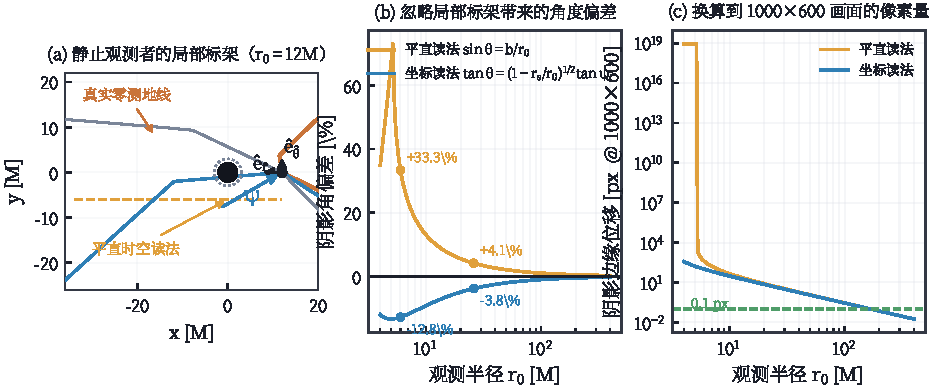
\includegraphics[width=0.99\linewidth]{figures/f14_observer_frame.pdf}
\caption{静态观测者标架与两种朴素读法的误差。(a) 观测者的径向与切向
基向量、真实零测地线与同冲击参数的平直线；(b) 两种朴素读法在不同
观测半径下的角度偏差；(c) 同一偏差换算到 $1000\times600$、
$\mathrm{fov}=58^\circ$ 的像素量，虚线为 $0.1$\,px 参考线。}
\label{fig:14}
\end{figure}

图~\ref{fig:14}(c) 是本节的实用结论：当 $r_0\gtrsim20\M$ 时，
两种朴素读法的像素误差都掉到 $0.1$\,px 以下，因此\emph{在这个距离以外
用哪种角都不会在画面上看出来}；但近距预设（$r_0=12\M$，
近观光子环）下平直读法会带来 $4.5$\,px 的阴影半径误差，
坐标读法带来 $-4.15$\,px，是肉眼可见的系统偏移。
模拟器统一采用式~\eqref{eq:fidoang}，因此在全部预设下自洽。

% --------------------------------------------------------------------------- #
\subsection{V5：有限逃逸半径的出射方向误差}\label{sec:v5}

第五项验证针对一个必须做的近似：积分不可能推进到 $r\to\infty$，
模拟器在 $u<u_{\min}=1/\max(R_{\rm esc},1.6r_0)$ 且径向向外时
判定逃逸，并用式~\eqref{eq:escapedir} 的解析极限方向
$\vec t_{\rm dir}$ 采样背景。这等于假设「从 $R_{\rm esc}$ 到无穷远的
剩余偏折可以忽略」，而巴蒂亚（弱场）级数给出的剩余偏折角为
\begin{equation}
\Delta\psi_{\rm rem}\simeq \frac{2\rs}{R_{\rm esc}}
+\frac{15\pi}{4}\Bigl(\frac{\rs}{R_{\rm esc}}\Bigr)^{2}+\cdots,
\label{eq:remdef}
\end{equation}
对 $R_{\rm esc}=140\M$ 这只有 $2.1\times10^{-2}$\,rad 的量级，
再乘上背景星场在方向上的梯度，就是最终可见的误差。

%% generated by tools/make_tables.py -- do not edit
\begin{table}[t]
\centering
\caption{V5：有限逃逸半径 $R_{\rm esc}=140\,M$ 造成的出射方向误差（$1000\times600$、$\mathrm{fov}=58^{\circ}$ 下的像素量）。最大误差 $0.021$\,px，远小于一个像素。}
\label{tab:v5}
\small
\begin{tabular}{lrr}
\toprule
$b/M$ & 方向误差 [rad] & 像素误差 \\
\midrule
5.1962 & $2.764\times 10^{-7}$ & 0.00016 \\
6.0000 & $4.241\times 10^{-7}$ & 0.00025 \\
9.0000 & $1.427\times 10^{-6}$ & 0.00085 \\
14.0000 & $5.377\times 10^{-6}$ & 0.00319 \\
20.0000 & $1.573\times 10^{-5}$ & 0.00932 \\
26.0000 & $3.471\times 10^{-5}$ & 0.02057 \\
\bottomrule
\end{tabular}

\end{table}


表~\ref{tab:v5} 给出六个代表性冲击参数的实测方向误差：
从 $2.76\times10^{-7}$\,rad（$b=\bc$）到
$3.47\times10^{-5}$\,rad（$b=26\M$），
最大值换算为 $0.0206$\,px——比一个像素小 48 倍。
图~\ref{fig:17}(a) 把它放进完整的误差预算：默认参数下
离散化误差（$tol=10^{-3}$，$2.6\times10^{-3}$\,px）、
逃逸截断（$2.1\times10^{-2}$\,px）、单精度状态漂移
（$5.25\times10^{-8}$\,rad $=3.1\times10^{-5}$\,px）
与边缘像素量化（$0.5$\,px）之中，量化占绝对主导。
这不是坏事：它说明在 $1000\times600$ 一类的视口下，
限制精度的是\emph{采样}而非\emph{物理}，
这正是模拟器把预算投向累积与抗锯齿（\S\ref{sec:jitter}）而非
无限提高积分精度的原因。

\begin{figure}[t]
\centering
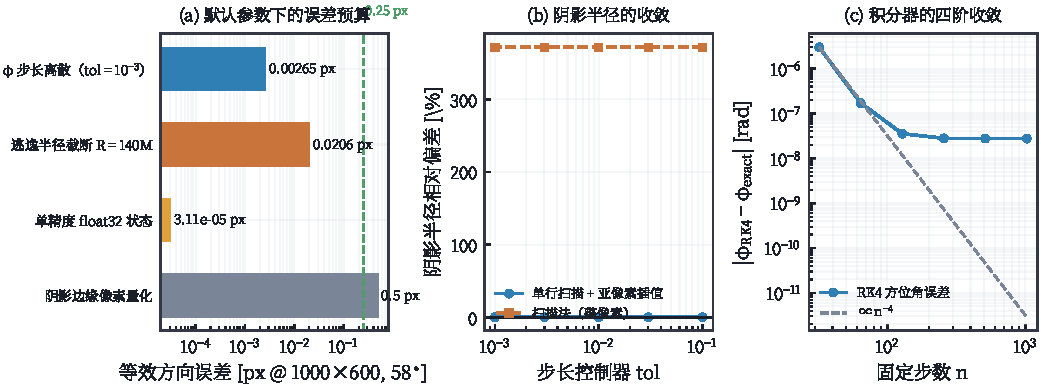
\includegraphics[width=0.99\linewidth]{figures/f17_error_budget.pdf}
\caption{误差预算与收敛性。(a) 默认参数下四类误差的等效像素大小；
(b) 阴影半径相对偏差随 $tol$ 的收敛，含整像素扫描与亚像素插值两种口径；
(c) 固定步数下方位角误差的 $n^{-4}$ 收敛。}
\label{fig:17}
\end{figure}

图~\ref{fig:17}(b) 值得单独说明：两条曲线在 $tol\lesssim10^{-2}$ 之后
几乎水平，说明\emph{阴影半径已经收敛}，剩下的 $-0.5$\,px 左右的
偏移不随 $tol$ 改善——它就是半像素量化。
这与 \S\ref{sec:termination} 末尾预告的「边缘锐利度与边缘位置
由不同机制控制」完全对应。

% --------------------------------------------------------------------------- #
\subsection{V6：累积、抖动与「同一配置是否给出同一张图」}\label{sec:v6}

前三类验证都在问「公式对不对」。第六项验证问的是另一个问题：
\textbf{当前这一帧里，那个像素值究竟平均了多少个彼此独立的样本？}
这不是一个哲学问题，而是一个可以用位（bit）来回答的问题，
而且本文恰好有一次失败的回答可供对照。

\paragraph{设计。}探针（\texttt{tools/validate\_accum.py}）把应用
驱到固定的 $560\times360$ 舞台（侧栏收起）、\texttt{renderScale}$=0.5$
（受追踪分辨率 $280\times180$）、\texttt{maxSteps}$=120$、$tol=0.06$、
坐标时间冻结在 $t=14\M$、\texttt{autoQuality} 关闭、暂停，
然后按倍增序列 $n=1,2,4,\dots,2048$ 各调用一次
\texttt{window.\_\_bh.accumulateTo(n)}：该接口内部强制暂停、
清零累积计数器、连续渲染 $n$ 帧、把 HDR 累积缓冲经过完整后处理写入
一块 LDR 缓冲并回读，同时返回抽稀网格与整条中央扫描行。
因此\textbf{每张被测图像的样本数是精确已知的}，
而截图做不到这一点——截图期间累积仍在继续。

三个块共享同一套几何与同一张 $n=N_{\rm ref}=2048$ 参考图：
\emph{frozen} 把抖动样本序号钉在 0（即 1.0.0 的行为）、
\emph{r2} 使用修好之后的低差异序列、\emph{post} 在 r2 之上再打开
发行版的全部后处理（\texttt{grain}$=0.010$、\texttt{vignette}$=0.35$）。
每块另在 $n=1$ 与 $n=64$ 上把\emph{同一个} $n$ 连着测两次，
两者之差即探针自身的\emph{可重复性下限}。

\paragraph{一个必须先排掉的混淆。}第一版探针给出的数字是错的，
而错误本身很有教益。它报告 frozen 块在 $n\ge2$ 处稳定在
$4.19\times10^{-3}$（luma 单位）而不是零，并且 $n=1$ 点
高达 $3.30\times10^{-2}$——约为平台的 8 倍。
三个原因层层叠加：（i）\texttt{autoQuality} 没关，
这台软光栅机器上块均帧率长时间低于 $24$\,fps，
于是 \texttt{renderScale} 在\emph{同一轮} schedule 的两次测量之间
被下调，重新分配了全部渲染目标，受追踪分辨率中途改变；
（ii）复合通道叠加的抖动用 $u_{\rm frame}=\texttt{frameCount}\bmod1024$
作相位，而 \texttt{frameCount} 是全局计数器，
\texttt{resetAccumulation()} 从不重置它，于是\emph{同一配置两次渲染
必然得到不同的抖动画幅}，在 8 位 luma 上直接压出一条
$3\times10^{-3}\sim4\times10^{-3}$ 的地板；
（iii）在一串 \texttt{set()} 之后的第一次 \texttt{accumulateTo()}
落在尚未稳定的管线上。修法是三项一起做：相位回归累积历元
（\S\ref{sec:jitter}）、探针关闭 \texttt{autoQuality} 与
\texttt{grain}/\texttt{vignette}、并在每块开始丢弃两帧暖机；
探针还会断言整轮 schedule 中受追踪分辨率与 \texttt{renderScale}
恒定，否则直接抛错。

\paragraph{结果。}表~\ref{tab:v6summary} 给出六项实验的汇总，
图~\ref{fig:24}(a) 把三块的 rms 随 $n$ 的走向画在同一对数横轴上。
四点结论：

\begin{enumerate}[leftmargin=1.5em,itemsep=2pt,topsep=3pt]
\item \textbf{frozen 块逐位相同。}把样本序号钉死之后，
12 个 $n$ 上的 rms \emph{恒等于} $0.000$，
$n=1$ 与 $n=2048$ 的中央行逐元素相同，
两次重复测量的 rms、行 rms 与最大差也都是 $0.000$。
这正是解析预期：如果每一帧都相同，任何算术平均都等于那一帧。
所以这一行是\textbf{对探针与累积路径的校验，不是对物理的校验}——
它证明「平均 $n$ 个相同的东西」确实是幂等的，
并因此让 $n=1$ 的旧值 $3.30\times10^{-2}$ 无所遁形。
\item \textbf{r2 块真的在平均不同的样本。}rms 从
$n=1$ 的 $5.44\times10^{-2}$ 单调降到 $n=1024$ 的
$6.02\times10^{-3}$，$n=N_{\rm ref}$ 处按定义为 0，
共降 $9.0$ 倍。相邻中心行样本差的均方（$h_{\rm f}$，
可读作残余高频能量）从 $1.081\times10^{-4}$ 降到
$7.86\times10^{-5}$，降 $27\%$：抖动把轮廓边缘与程序化星场的
亚像素结构真正抹平了一部分，而不只是把图移动了半个像素。
\item \textbf{收敛慢于独立采样。}若 $n$ 帧互相独立，
应有 $\mathrm{rms}\propto n^{-1/2}$；对 $n=1\ldots1024$
做对数—对数回归得到的是 $n^{-0.29}$（r2）与 $n^{-0.28}$（post）。
这不是实现缺陷，而是这条曲线的定义使然：
\texttt{accumulateTo(n)} 每次都从第 1 帧重放\emph{同一条}
确定性 R2 序列，于是 $\bar f_n$ 是同一序列的前缀，
相邻两个前缀高度相关；同时参考图本身只有 $2048$ 个样本，
而方差集中在轮廓处的\emph{不连续}覆盖率积分与 8 位量化上。
因此这个指数是\textbf{该度量的性质}，不能读作渲染器的收敛阶。
\item \textbf{相位修复使「暂停即定帧」。}post 块在
\texttt{grain}$=0.010$ 全部打开的情况下，
$n=1$ 与 $n=64$ 的重复对 rms、行 rms、最大差\emph{全部为} $0.000$；
修复前同口径的下限约 $4\times10^{-3}$。这与 \S\ref{sec:v6}
开头列出的（ii）完全对应：胶片颗粒是\emph{累积之后}由复合通道
按历元相位叠加的，任何 $n$ 都平均不掉它，
但它现在对同一配置是\emph{确定且可重复}的——
这正是「静止画面应该看起来稳定」所需要的性质。
\end{enumerate}

\paragraph{耗时口径。}post 块在 $n=2048$ 上耗时 $45.6$\,s，
r2 块 $47.6$\,s、frozen 块 $48.2$\,s；把 $n\ge64$ 的五个测点
除以 $n$ 得每帧 $23.3\sim25.4$\,ms（离散度 $<5\%$，
受机器计时器量化限制，见 \S\ref{sec:perf}），
而 $n=1$ 的 $0.186$\,s 中约 $0.16$\,s 是与 $n$ 无关的
固定开销（\texttt{glReadPixels} 回读 $560\times360$ 加一次强制同步）。
换言之：累积成本对 $n$ 是线性的，这是把「渐进渲染」
变成可预算特性的前提。

\begin{figure}[t]
\centering
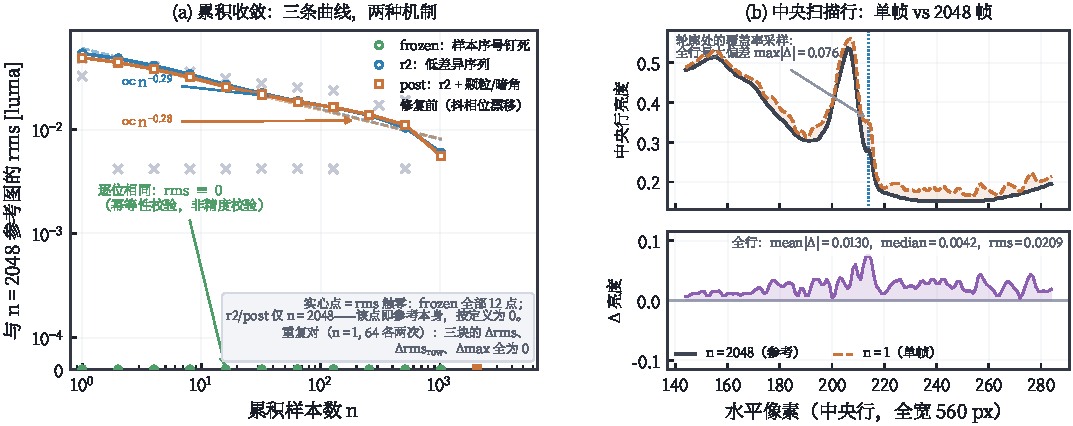
\includegraphics[width=0.99\linewidth]{figures/f24_accumulation.pdf}
\caption{累积管线的收敛性与相位一致性。(a) 三个块相对各自
$n=2048$ 参考图的 rms 随 $n$ 的变化（双对数轴）：frozen 块
（样本序号钉死）恒为 0 的「地平线」，r2 块（低差异序列）的单调下降，
以及打开全部后处理的 post 块；淡灰叉号为\emph{修复前}的旧数据
（其 schedule 只到 $n=4096$，且平台由抖相位漂移造成）。
(b) 中央扫描行的局部放大：$n=1$ 与参考图的亮度剖面。}
\label{fig:24}
\end{figure}

\paragraph{诚实边界。}本节的结论严格限于三点：
frozen 地平线验证的是「幂等」而非精度；r2 与 post 的下降由
\emph{同一}确定性序列的前缀差异驱动，因而不是无偏的
蒙特卡洛误差估计；$n=N_{\rm ref}$ 处 rms 为 0 是度量的定义，
不是「误差为零」。真正可外推的是（i）每帧成本与 $n$ 成正比、
（ii）同一配置的重复渲染逐位相同、（iii）残余高频能量随 $n$ 单调下降
——这三条恰好就是「渐进累积」这一交互范式要求的全部内容。

% --------------------------------------------------------------------------- %
\subsection{六项实验的汇总}\label{sec:vsum}

表~\ref{tab:v6summary} 把 V1--V6 的对照量、误差与判据集中列出。
判据一栏是本文采用的验收标准：几何量须在双精度舍入水平内与闭式一致，
渲染量须在亚像素内一致，管线量须在量化台阶内不可区分。
凡是未达标的项都在下方备注栏中说明其物理或数值来源。

%% generated by tools/make_tables.py -- do not edit
\begin{table}[t]
\centering
\caption{六项验证实验的汇总。``对照量'' 一栏给出该项所对照的闭式解或参考实现，``偏差'' 一栏为实测值与参照值之差（相对量以百分数或科学计数法给出）。判据一栏是本文采用的验收标准：几何量须在双精度舍入水平内与闭式一致，渲染量须在亚像素内一致，管线量须在量化台阶内不可区分。末列为相应的物理或数值说明；全部数值由 \protect\path{validate_pytrace.json} 与 \protect\path{validate_accum.json} 经 \protect\path{tools/make_tables.py} 生成。}
\label{tab:v6summary}
\scriptsize
\begin{tabular}{l p{0.18\linewidth} p{0.15\linewidth} p{0.09\linewidth} p{0.17\linewidth} p{0.20\linewidth}}
\toprule
\# & 对照量 & 关键实测 & 偏差 & 判据 & 备注 \\
\midrule
V1 & 临界冲击参数 $b_{c}=3\sqrt{3}\,M$ & $b_{\rm edge}=5.196152422707$ & $9.99\times 10^{-15}$ & $|\Delta b|/b_{c}<10^{-12}$ & 二分搜索在双精度舍入极限处闭合 \\
V2 & 近临界轨道守恒性（$b=5.196147418$，绕光子球 $15.05$\,rad） & $\max$ 残差 $2.62\times 10^{-6}$ & 较 $tol=10^{-2}$ 下降 $159\times$ & 残差在 $tol\le 3\times10^{-4}$ 处触底 & 触底值为机器精度，继续收紧容差无改善 \\
V3 & 阴影半径的像素映射（闭式 $f_{\rm px}\tan\psi_{\rm sh}$） & $R_{\rm px}$ 亚像素反解 & $6.48\times 10^{-12}$ & 亚像素 $<10^{-9}$；整数扫描 $<1$\,px & 扫描口径的 0.84\% 偏差是像素量化，非物理误差 \\
V4a & 屏幕纵坐标 $\to$ 冲击参数 $b$ 的闭式 & $b_{\rm tracer}=12.08060346$ & $4.44\times 10^{-16}$ & $<10^{-12}$ & 几何映射与着色器实现逐位一致 \\
V4b & FIDO 角半径 $\sin\psi=(3\sqrt{3}M/r_{0})$ $\sqrt{1-2M/r_{0}}$ & $r_{0}=4M$：$\psi=66.716^{\circ}$ & $+34.90\%$ & FIDO 口径为准；flat/chart 均为近似 & 同一行 chart 口径 $-12.05\%$；$r_{0}\ge26M$ 后两口径误差才降到 $5\%$ 内 \\
V5 & 逃逸半径处的出射方向重建 & $\max=0.0206$\,px @ $1000\times600$ & -- & $<0.05$\,px & 误差随 $b$ 单调增长；$R_{\rm esc}=140M$ 在此视场下足够 \\
V6 & 渐进累积收敛（$n=1\to1024$，逐位重复） & rms 降 $9.04$ 倍，$\propto n^{-0.29}$ & -- & 8-bit 亮度地板 $=0$；三块重复对逐位相同 & 窗口内高频残余：r2 降 $24.5\%$，post 降 $14.8\%$ \\
V6 & 幂等性对照（$\Delta\equiv0$） & 重复对最大差异 $0.0$ & $0$ & 同一配置重复渲染须逐位相同 & 冻结抖动时 rms $\equiv0$：这是幂等性校验，不是精度校验 \\
\bottomrule
\end{tabular}

\end{table}

